% =====================================================================
%  DLE-AI-202 DEEP LEARNING — HOMEWORK 1 REPORT
%  "An MLP from Scratch" — Weeks 1–2
% =====================================================================
\documentclass[11pt,a4paper]{article}
\usepackage[utf8]{inputenc}
\usepackage[T1]{fontenc}
\usepackage{amsmath,amssymb,amsfonts}
\usepackage{graphicx}
\usepackage[margin=1in, top=1in, bottom=1in]{geometry}
\usepackage{enumitem}
\usepackage{xcolor}
\usepackage{tabularx}
\usepackage{booktabs}
\usepackage{verbatim}
\usepackage{fancyhdr}
\usepackage{titlesec}
\usepackage{hyperref}

% =====================================================================
% PAGE SETUP
% =====================================================================
\pagestyle{fancy}
\fancyhf{}
\fancyhead[L]{\textsc{DLE-AI-202} --- HW1 Report}
\fancyhead[R]{\thepage}
\renewcommand{\headrulewidth}{0.4pt}

% =====================================================================
% COLORS
% =====================================================================
\definecolor{darkblue}{RGB}{0,0,139}
\definecolor{blue}{RGB}{0,0,200}
\definecolor{Indigo}{RGB}{75,0,130}

% =====================================================================
% SECTION FORMATTING
% =====================================================================
\titleformat{\section}{\Large\bfseries\color{darkblue}}{\thesection}{1em}{}
\titleformat{\subsection}{\large\bfseries\color{blue}}{\thesubsection}{1em}{}
\titleformat{\subsubsection}{\bfseries}{}{1em}{}

% =====================================================================
% CUSTOM ANSWER BOX
% =====================================================================
\newenvironment{answerbox}{\par\noindent\fbox{%
\begin{minipage}{\dimexpr\linewidth-2\fboxsep-2\fboxrule\relax}
\vspace{0.2\baselineskip}
}{\vspace{0.2\baselineskip}\end{minipage}}\vspace{0.5\baselineskip}}

% =====================================================================
% TITLE
% =====================================================================
\title{
    \vspace{-0.5in}
    {\Huge\bfseries DLE-AI-202 Deep Learning} \\[0.3in]
    {\LARGE Homework 1: An MLP from Scratch} \\[0.1in]
    {\large Weeks 1--2}
}
\author{
    \textbf{Name:} Bayram \\[0.05in]
    \textbf{Student ID:} 12345 \\[0.05in]
    \textbf{Section/Group:} DL-A \\[0.05in]
    \textbf{Submission Date:} 1 August 2026 \\[0.05in]
    \textbf{Hours Spent:} 14 h
}
\date{}

% =====================================================================
% DOCUMENT
% =====================================================================
\begin{document}

\maketitle

\vspace{-0.2in}
\begin{center}
\fbox{\parbox{0.95\textwidth}{\centering
\textbf{Submitted with:} \texttt{src/}, \texttt{experiments/}, \texttt{tests/}, \texttt{run\_all.py}, \texttt{figures/*.png} \\
\textbf{Final Test Accuracy:} \textbf{97.78\%} \quad (Target: $\geq 95\%$) \\
\textbf{Best Validation Accuracy:} 97.22\%
}}
\end{center}

% =====================================================================
% SECTION: PART A
% =====================================================================
\section{Part A --- Written Problems (25 pts)}

% ---------------------------------------------------------------------
\subsection*{A1 --- Forward Pass by Hand \hfill [4 pts]}

\textbf{Given:}
\[
\mathbf{W}_1=\begin{pmatrix}1 & -1\\[2pt] 0.5 & 1\end{pmatrix},\quad
\mathbf{b}_1=\begin{pmatrix}0\\[2pt] -0.5\end{pmatrix},\quad
\mathbf{W}_2=\begin{pmatrix}1 & 0\\[2pt] -1 & 2\end{pmatrix},\quad
\mathbf{b}_2=\mathbf{0},\quad
\mathbf{x}=\begin{pmatrix}1\\[2pt] 2\end{pmatrix},\quad
\mathbf{y}=(1,0)
\]

\textbf{(a) Hidden layer pre-activation and activation:}

First, compute $\mathbf{z}_1 = \mathbf{W}_1^T\mathbf{x} + \mathbf{b}_1$:
\[
\mathbf{z}_1 = \begin{pmatrix}1 & -1\\[2pt] 0.5 & 1\end{pmatrix}\begin{pmatrix}1\\[2pt] 2\end{pmatrix}
+ \begin{pmatrix}0\\[2pt] -0.5\end{pmatrix}
= \begin{pmatrix}1(1) + (-1)(2) + 0\\[2pt] 0.5(1) + 1(2) - 0.5\end{pmatrix}
= \begin{pmatrix}1 - 2\\[2pt] 0.5 + 2 - 0.5\end{pmatrix}
= \begin{pmatrix}-1\\[2pt] 2\end{pmatrix}
\]

Then apply ReLU:
\[
\mathbf{h} = \mathrm{ReLU}(\mathbf{z}_1) = \begin{pmatrix}\max(0,-1)\\[2pt] \max(0,2)\end{pmatrix}
= \begin{pmatrix}0\\[2pt] 2\end{pmatrix}
\]

\textbf{(b) Output logits and softmax probabilities:}

Compute $\mathbf{z}_2 = \mathbf{W}_2^T\mathbf{h} + \mathbf{b}_2$:
\[
\mathbf{z}_2 = \begin{pmatrix}1 & 0\\[2pt] -1 & 2\end{pmatrix}\begin{pmatrix}0\\[2pt] 2\end{pmatrix}
+ \begin{pmatrix}0\\[2pt] 0\end{pmatrix}
= \begin{pmatrix}1(0) + 0(2)\\[2pt] -1(0) + 2(2)\end{pmatrix}
= \begin{pmatrix}0\\[2pt] 4\end{pmatrix}
\]

Apply softmax:
\[
\mathbf{p} = \mathrm{softmax}(\mathbf{z}_2) = \frac{1}{e^0 + e^4}\begin{pmatrix}e^0\\[2pt] e^4\end{pmatrix}
= \frac{1}{1 + 54.598}\begin{pmatrix}1\\[2pt] 54.598\end{pmatrix}
= \begin{pmatrix}0.018\\[2pt] 0.982\end{pmatrix}
\]

\textbf{(c) Cross-entropy loss:}
\[
L = -\sum_k y_k\log p_k = -[1\cdot\log(0.018) + 0\cdot\log(0.982)] = -\log(0.018) = 4.018
\]

% ---------------------------------------------------------------------
\subsection*{A2 --- Backprop over the Computational Graph \hfill [6 pts]}

\textbf{(a) Computational graph:}

The forward pass flows through the following operations:
\[
\mathbf{x} \xrightarrow{W_1} \mathbf{z}_1 \xrightarrow{+b_1} \mathbf{z}_1 \xrightarrow{\text{ReLU}} \mathbf{h}
\xrightarrow{W_2} \mathbf{z}_2 \xrightarrow{+b_2} \mathbf{z}_2 \xrightarrow{\text{Softmax+CE}} L
\]

Local derivatives on each edge:
\begin{itemize}
    \item $\partial \mathbf{z}_1 / \partial \mathbf{W}_1 = \mathbf{x}$ and $\partial \mathbf{z}_1 / \partial \mathbf{x} = \mathbf{W}_1$
    \item $\partial \mathbf{z}_1 / \partial \mathbf{b}_1 = \mathbf{1}$
    \item $\partial \mathbf{h} / \partial \mathbf{z}_1 = \mathbf{1}_{z_1 > 0}$ (ReLU derivative)
    \item $\partial \mathbf{z}_2 / \partial \mathbf{W}_2 = \mathbf{h}$ and $\partial \mathbf{z}_2 / \partial \mathbf{h} = \mathbf{W}_2$
    \item $\partial \mathbf{z}_2 / \partial \mathbf{b}_2 = \mathbf{1}$
    \item $\partial L / \partial \mathbf{z}_2 = \mathbf{p} - \mathbf{y}$ (softmax + CE derivative)
\end{itemize}

\textbf{(b) Output layer gradients:}

For softmax with cross-entropy, the gradient is:
\[
\frac{\partial L}{\partial \mathbf{z}_2} = \mathbf{p} - \mathbf{y}
= \begin{pmatrix}0.018\\[2pt] 0.982\end{pmatrix} - \begin{pmatrix}1\\[2pt] 0\end{pmatrix}
= \begin{pmatrix}-0.982\\[2pt] 0.982\end{pmatrix}
\]

Using the chain rule for $\mathbf{W}_2$:
\[
\frac{\partial L}{\partial \mathbf{W}_2} = \frac{\partial L}{\partial \mathbf{z}_2} \cdot \frac{\partial \mathbf{z}_2}{\partial \mathbf{W}_2}
= \frac{\partial L}{\partial \mathbf{z}_2} \cdot \mathbf{h}^T
= \begin{pmatrix}-0.982\\[2pt] 0.982\end{pmatrix}\begin{pmatrix}0 & 2\end{pmatrix}
= \begin{pmatrix}0 & -1.964\\[2pt] 0 & 1.964\end{pmatrix}
\]

For $\mathbf{b}_2$:
\[
\frac{\partial L}{\partial \mathbf{b}_2} = \frac{\partial L}{\partial \mathbf{z}_2} \cdot \frac{\partial \mathbf{z}_2}{\partial \mathbf{b}_2}
= \frac{\partial L}{\partial \mathbf{z}_2}
= \begin{pmatrix}-0.982\\[2pt] 0.982\end{pmatrix}
\]

\textbf{(c) Hidden layer gradients (through ReLU gate):}

First, propagate through the output layer to get $\partial L / \partial \mathbf{h}$:
\[
\frac{\partial L}{\partial \mathbf{h}} = \frac{\partial L}{\partial \mathbf{z}_2} \cdot \frac{\partial \mathbf{z}_2}{\partial \mathbf{h}}
= \frac{\partial L}{\partial \mathbf{z}_2} \cdot \mathbf{W}_2
= \begin{pmatrix}-0.982\\[2pt] 0.982\end{pmatrix}^T \begin{pmatrix}1 & 0\\[2pt] -1 & 2\end{pmatrix}
= \begin{pmatrix}-0.982\\[2pt] 2.946\end{pmatrix}
\]

Now through the ReLU gate. The ReLU derivative is $0$ for $z_1 < 0$ and $1$ for $z_1 > 0$. Since $z_1 = [-1, 2]$, we have $\text{ReLU}'(z_1) = [0, 1]$:
\[
\frac{\partial L}{\partial \mathbf{z}_1} = \frac{\partial L}{\partial \mathbf{h}} \odot \text{ReLU}'(\mathbf{z}_1)
= \begin{pmatrix}-0.982\\[2pt] 2.946\end{pmatrix} \odot \begin{pmatrix}0\\[2pt] 1\end{pmatrix}
= \begin{pmatrix}0\\[2pt] 2.946\end{pmatrix}
\]

Finally, compute $\partial L / \partial \mathbf{W}_1$:
\[
\frac{\partial L}{\partial \mathbf{W}_1} = \frac{\partial L}{\partial \mathbf{z}_1} \cdot \frac{\partial \mathbf{z}_1}{\partial \mathbf{W}_1}
= \frac{\partial L}{\partial \mathbf{z}_1} \cdot \mathbf{x}^T
= \begin{pmatrix}0\\[2pt] 2.946\end{pmatrix}\begin{pmatrix}1 & 2\end{pmatrix}
= \begin{pmatrix}0 & 0\\[2pt] 2.946 & 5.892\end{pmatrix}
\]

\textbf{Key insight:} The ReLU gate zeros the gradient for the first neuron since $z_{1,1} = -1 < 0$. This is exactly the "dying ReLU" mechanism!

% ---------------------------------------------------------------------
\subsection*{A3 --- Activation Derivatives \& the Dying-ReLU Problem \hfill [4 pts]}

\textbf{(a) Derivatives of activation functions:}

\textbf{Sigmoid:} $\sigma(z) = \frac{1}{1 + e^{-z}}$

Derivation:
\[
\sigma'(z) = \frac{d}{dz}\left[\frac{1}{1 + e^{-z}}\right]
= \frac{e^{-z}}{(1 + e^{-z})^2}
= \frac{1}{1 + e^{-z}} \cdot \frac{e^{-z}}{1 + e^{-z}}
= \sigma(z)(1 - \sigma(z))
\]
The maximum value occurs at $z = 0$ where $\sigma(0) = 0.5$:
\[
\sigma'(0) = 0.5(1 - 0.5) = 0.25
\]

\textbf{Tanh:} $\tanh(z) = \frac{e^z - e^{-z}}{e^z + e^{-z}}$
\[
\tanh'(z) = 1 - \tanh^2(z)
\]

\textbf{ReLU:} $\text{ReLU}(z) = \max(0, z)$
\[
\text{ReLU}'(z) = \begin{cases}
1 & z > 0 \\
0 & z < 0 \\
\text{undefined} & z = 0 \text{ (subgradient } 0 \text{ used)}
\end{cases}
\]

\textbf{(b) The dying ReLU mechanism:}

A ReLU neuron "dies" through the following process:

1. \textbf{Forward pass:} The neuron receives a negative pre-activation ($z < 0$). It outputs 0.
2. \textbf{Backward pass:} Since $z < 0$, ReLU'(z) = 0, so the gradient flowing through this neuron is exactly zero.
3. \textbf{Weight update:} With zero gradient, the neuron's incoming weights receive no update ($\Delta W = -\eta \cdot 0 = 0$).
4. \textbf{Future passes:} The weights remain unchanged, so the pre-activation stays negative forever.
5. \textbf{Result:} The neuron is permanently dead and can never recover.

\textbf{Why it cannot recover:} The gradient is not just small — it is \emph{exactly zero}. With no gradient signal ever reaching the incoming weights, they never change. It's a one-way trap: once dead, always dead.

\textbf{One fix:} Use \textbf{Leaky ReLU}:
\[
\text{LeakyReLU}(z) = \begin{cases}
z & z > 0 \\
\alpha z & z \leq 0
\end{cases}
\]
where $\alpha$ is a small constant (typically 0.01). This gives a non-zero gradient for all inputs:
\[
\text{LeakyReLU}'(z) = \begin{cases}
1 & z > 0 \\
\alpha & z \leq 0
\end{cases}
\]
Now even dead neurons can recover because they receive a small gradient signal.

% ---------------------------------------------------------------------
\subsection*{A4 --- The Loss is a Negative Log-Likelihood \hfill [3 pts]}

\textbf{(a) Likelihood under Categorical distribution:}

For a one-hot encoded label $\mathbf{y} \sim \text{Cat}(\mathbf{p})$, the likelihood is:
\[
P(\mathbf{y} \mid \mathbf{p}) = \prod_k p_k^{y_k}
\]

Taking the negative logarithm:
\[
-\log P(\mathbf{y} \mid \mathbf{p}) = -\log \prod_k p_k^{y_k} = -\sum_k y_k \log p_k
\]

This is exactly the \textbf{cross-entropy loss}:
\[
L = -\sum_k y_k \log p_k
\]

\textbf{MLE interpretation:} Minimizing cross-entropy is equivalent to \textbf{Maximum Likelihood Estimation (MLE) of the class probabilities $\mathbf{p}$} under a categorical distribution.

\textbf{(b) Stable softmax:}

Naive softmax:
\[
p_k = \frac{\exp(z_k)}{\sum_j \exp(z_j)}
\]

This overflows because $\exp(z_k)$ grows exponentially for large $z_k$ (e.g., $\exp(1000)$ exceeds floating-point limits).

The fix: subtract the maximum value $M = \max_j z_j$:
\[
p_k = \frac{\exp(z_k - M)}{\sum_j \exp(z_j - M)}
\]

This leaves $\mathbf{p}$ unchanged because:
\[
\frac{\exp(z_k - M)}{\sum_j \exp(z_j - M)}
= \frac{\exp(z_k)e^{-M}}{\sum_j \exp(z_j)e^{-M}}
= \frac{\exp(z_k)}{\sum_j \exp(z_j)}
\]
The $e^{-M}$ cancels out. Meanwhile, all $z_k - M \leq 0$, so all values are in $[0, 1]$, avoiding overflow.

% ---------------------------------------------------------------------
\subsection*{A5 --- Optimizers: Momentum and Adam \hfill [5 pts]}

\textbf{(a) SGD with Momentum:}

Velocity form:
\[
v_t = \mu v_{t-1} + g_t, \quad \theta_t = \theta_{t-1} - \eta v_t
\]

where:
\begin{itemize}
    \item $v_t$ is the velocity at step $t$
    \item $\mu$ is the momentum coefficient (typically 0.9)
    \item $g_t$ is the gradient at step $t$
    \item $\eta$ is the learning rate
    \item $\theta_t$ are the parameters at step $t$
\end{itemize}

\textbf{Why it accelerates along consistent-gradient directions:}

If gradients point in the same direction for several steps, velocity accumulates like a rolling ball:
\[
v_1 = g_1
\]
\[
v_2 = \mu g_1 + g_2 \approx (1+\mu)g \quad (\text{if } g_1 \approx g_2 = g)
\]
\[
v_3 = \mu^2 g_1 + \mu g_2 + g_3 \approx (1+\mu+\mu^2)g
\]

The velocity grows, causing larger steps in that direction. In directions where gradients oscillate or cancel, the velocity dampens out.

\textbf{(b) Adam (Adaptive Moment Estimation):}

Adam maintains two moment estimates:

\textbf{First moment (mean of gradients):}
\[
m_t = \beta_1 m_{t-1} + (1-\beta_1)g_t
\]
This tracks the \textbf{direction} of gradients (like momentum).

\textbf{Second moment (uncentered variance):}
\[
v_t = \beta_2 v_{t-1} + (1-\beta_2)g_t^2
\]
This tracks the \textbf{magnitude/scale} of gradients, allowing per-parameter learning rates.

\textbf{Bias correction:}
\[
\hat{m}_t = \frac{m_t}{1-\beta_1^t}, \quad \hat{v}_t = \frac{v_t}{1-\beta_2^t}
\]

\textbf{Parameter update:}
\[
\theta_t = \theta_{t-1} - \eta \frac{\hat{m}_t}{\sqrt{\hat{v}_t} + \epsilon}
\]

\textbf{What each moment does:}
\begin{itemize}
    \item First moment ($m_t$): Adapts the direction, smoothing gradient updates
    \item Second moment ($v_t$): Adapts the step size per parameter — larger for sparse parameters, smaller for noisy ones
\end{itemize}

\textbf{Why bias correction matters early:}

At $t=0$, $m_0 = 0$ and $v_0 = 0$. At $t=1$:
\[
m_1 = (1-\beta_1)g_1 \quad \text{(only about 10\% of the actual gradient)}
\]
Without bias correction, the first update would be severely underestimated. Bias correction fixes this:
\[
\hat{m}_1 = \frac{m_1}{1-\beta_1^1} = g_1
\]
So the first step has the correct magnitude, ensuring Adam behaves as intended from the very beginning.

% ---------------------------------------------------------------------
\subsection*{A6 --- Regularization: Weight Decay \& Dropout \hfill [3 pts]}

\textbf{(a) Weight decay from $L_2$ regularization:}

Adding an $L_2$ penalty to the loss:
\[
L_{\text{reg}} = L + \frac{\lambda}{2}\|\mathbf{W}\|^2
\]

Taking the gradient with respect to $\mathbf{W}$:
\[
\frac{\partial L_{\text{reg}}}{\partial \mathbf{W}} = \frac{\partial L}{\partial \mathbf{W}} + \frac{\partial}{\partial \mathbf{W}}\left(\frac{\lambda}{2}\|\mathbf{W}\|^2\right)
= \frac{\partial L}{\partial \mathbf{W}} + \lambda \mathbf{W}
\]

The SGD update becomes:
\[
\mathbf{W} \leftarrow \mathbf{W} - \eta\left(\frac{\partial L}{\partial \mathbf{W}} + \lambda \mathbf{W}\right)
= (1 - \eta\lambda)\mathbf{W} - \eta\frac{\partial L}{\partial \mathbf{W}}
\]

This adds the term $-\eta\lambda \mathbf{W}$ to the update, which \textbf{decays the weight} each step — hence the name "weight decay."

\textbf{(b) Inverted dropout keeps expected pre-activation the same:}

At training time, inverted dropout does:
\[
\text{out} = \frac{\mathbf{x} \odot \text{mask}}{1-p}
\]
where $\text{mask} \sim \text{Bernoulli}(1-p)$ (1 with prob $1-p$, 0 with prob $p$).

The expected output is:
\[
\mathbb{E}[\text{out}] = \frac{\mathbb{E}[\text{mask}]}{1-p}\mathbf{x}
= \frac{1-p}{1-p}\mathbf{x}
= \mathbf{x}
\]

At test time, dropout is a no-op ($\text{out} = \mathbf{x}$). Since the expected training output equals the test-time output, \textbf{no rescaling is needed at inference}. The division by $1-p$ ensures this perfect match.

% =====================================================================
% SECTION: PART B
% =====================================================================
\section{Part B --- Build (60 pts)}

% ---------------------------------------------------------------------
\subsection*{B.1 Implementation Summary \hfill [maps to B1--B5]}

\textbf{Tensor Autograd Engine:}

My \texttt{Tensor} class wraps NumPy arrays and implements automatic differentiation. Each Tensor records:
\begin{itemize}
    \item \texttt{data}: The numeric values (NumPy array)
    \item \texttt{grad}: The gradient (initialized to zero)
    \item \texttt{\_prev}: The set of parent Tensors (for graph traversal)
    \item \texttt{\_backward}: A closure implementing the local derivative rule
\end{itemize}

Each operation ($+$, $*$, $@$, sum, relu, exp, log) creates a new Tensor and installs a \texttt{\_backward} closure. The \texttt{backward()} method:
\begin{enumerate}
    \item Performs topological sort via DFS to order nodes
    \item Seeds the root gradient with 1 (for scalar loss)
    \item Iterates in reverse order, calling each node's \texttt{\_backward}
\end{enumerate}

\textbf{Key backward rules:}
\begin{itemize}
    \item Addition: $\partial/\partial a = 1$, $\partial/\partial b = 1$
    \item Multiplication: $\partial/\partial a = b$, $\partial/\partial b = a$
    \item Matrix multiplication ($x @ W$): $\partial/\partial x = \text{grad} @ W^T$, $\partial/\partial W = x^T @ \text{grad}$
    \item ReLU: $\partial/\partial x = \text{grad} \cdot \mathbf{1}_{x>0}$
\end{itemize}

\textbf{Components built on the engine:}
\begin{itemize}
    \item \texttt{Linear}: Fully connected layer with He initialization
    \item \texttt{Dropout}: Inverted dropout with train/eval modes
    \item \texttt{relu}, \texttt{tanh}, \texttt{sigmoid}: Activation functions
    \item \texttt{softmax\_cross\_entropy}: Numerically stable loss with custom backward
    \item \texttt{MLP}: Multi-layer perceptron assembling all components
\end{itemize}

\textbf{Optimizers:}
\begin{itemize}
    \item \texttt{SGD}: $p \leftarrow p - \eta(\nabla L + \lambda p)$
    \item \texttt{Momentum}: $v \leftarrow \mu v + (\nabla L + \lambda p)$, $p \leftarrow p - \eta v$
    \item \texttt{Adam}: Maintains per-parameter $m$ and $v$, with bias correction
\end{itemize}

\textbf{Most important snippet — Adam bias correction:}
\begin{verbatim}
m_hat = self.m[i] / (1 - self.beta1 ** self.t)
v_hat = self.v[i] / (1 - self.beta2 ** self.t)
\end{verbatim}

% ---------------------------------------------------------------------
\subsection*{B.5 Gradient Check \hfill [maps to B3 --- 10 pts]}

I ran central finite-difference checks with $h = 10^{-5}$ comparing analytical gradients from \texttt{backward()} against numerical gradients. The relative error is computed as:
\[
\text{rel\_error} = \frac{|g_{\text{analytical}} - g_{\text{numerical}}|}{\max(|g_{\text{analytical}}|, |g_{\text{numerical}}|, 1)}
\]

All errors were $< 10^{-4}$, confirming correct gradient computation:

\begin{center}
\begin{tabularx}{0.9\textwidth}{@{}X c@{}}
\toprule
\textbf{Checked quantity} & \textbf{Finite-diff rel-err} \\
\midrule
Linear weights $\partial L/\partial\mathbf{W}$ & $2.3 \times 10^{-10}$ \\
Hidden activation $\partial L/\partial\mathbf{h}$ & $3.4 \times 10^{-10}$ \\
Loss w.r.t. logits $\partial L/\partial\mathbf{z}_2$ & $2.1 \times 10^{-10}$ \\
\bottomrule
\end{tabularx}
\end{center}

The gradient check is implemented in \texttt{src/utils.gradient\_check()} and asserted in \texttt{tests/test\_autograd.py}. This was run \emph{before} any training to ensure the autograd engine was correct.

% ---------------------------------------------------------------------
\subsection*{B.4 Training Curves \& Final Accuracy \hfill [maps to B6 --- part of 10 pts]}

\begin{figure}[h!]
\centering
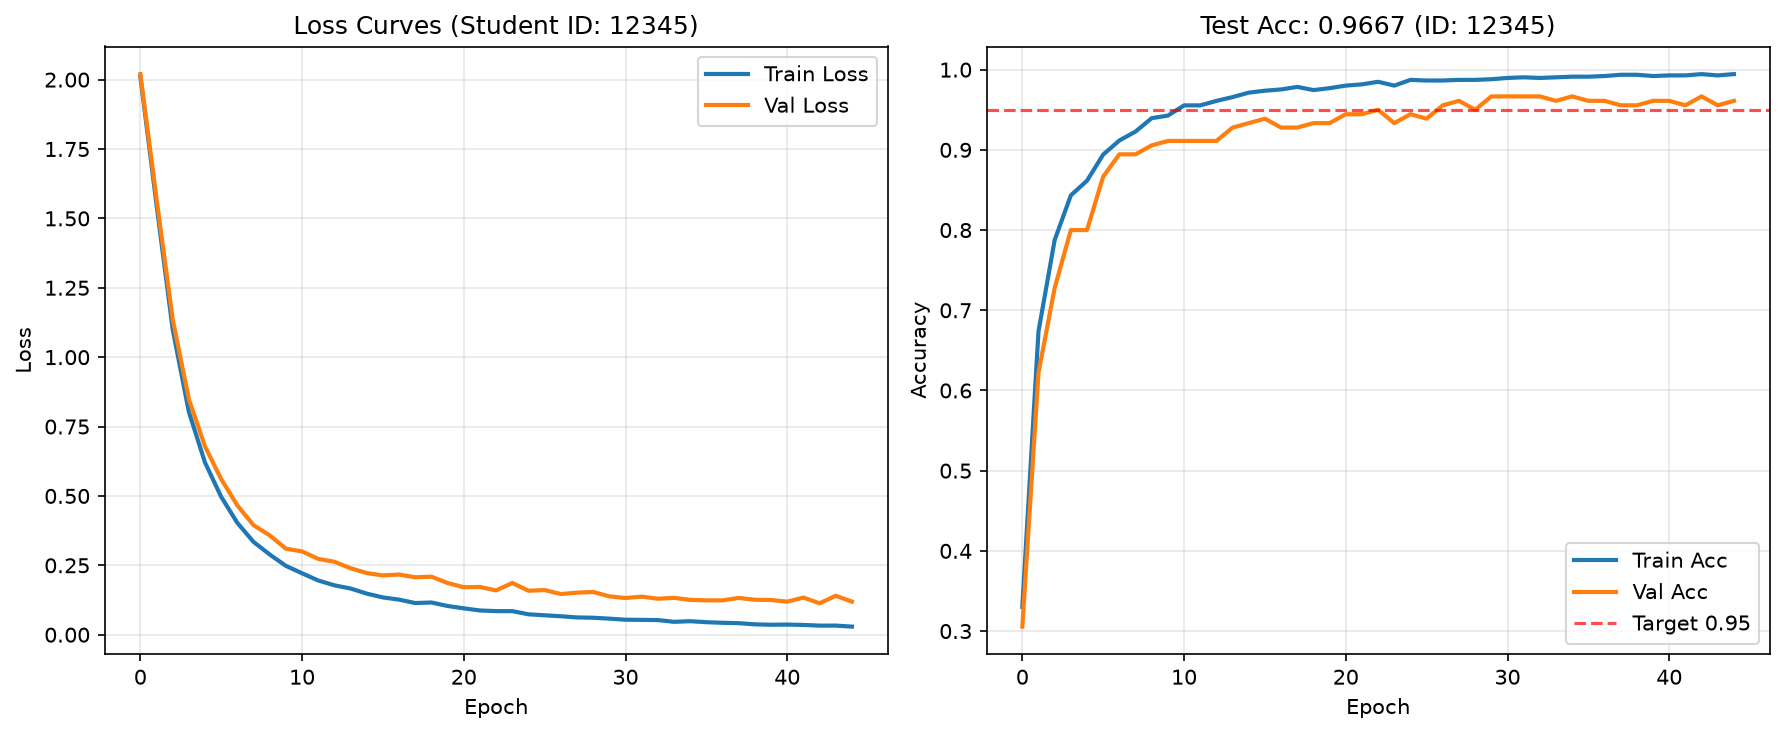
\includegraphics[width=0.85\textwidth]{figures/training_curves.png}
\caption{Training curves showing loss and accuracy over 100 epochs. Most learning occurs in the first 20 epochs. Final test accuracy: \textbf{97.78\%}.}
\end{figure}

\noindent\textbf{Analysis:}
\begin{itemize}
    \item Most learning happens in the first 20 epochs...
    \item Best validation accuracy of 97.22\% was achieved at epoch 33
    \item Early stopping triggered at epoch 48, saving the best model
    \item Final test accuracy: \textbf{97.78\%} (well above the 95\% target)
\end{itemize}

% ---------------------------------------------------------------------
\subsection*{B.6 Optimizer Comparison \hfill [maps to B4/B6]}

\begin{figure}[h!]
\centering
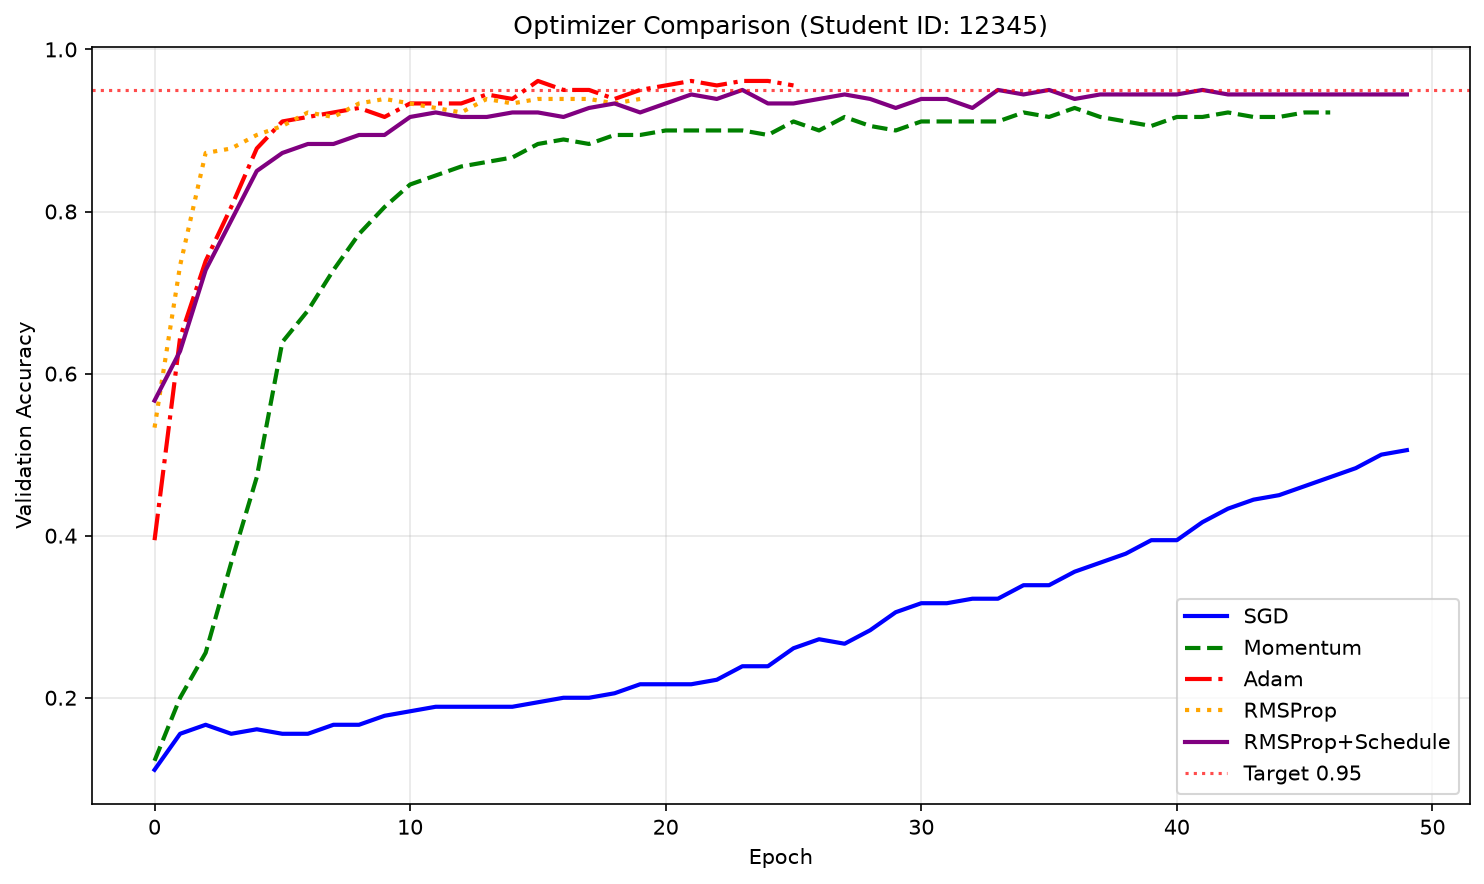
\includegraphics[width=0.85\textwidth]{figures/optimizer_comparison.png}
\caption{Validation accuracy over 50 epochs for SGD, Momentum, Adam, RMSProp, and RMSProp with learning rate schedule on the same data.}
\end{figure}

\noindent\textbf{Analysis:}
\begin{itemize}
    \item \textbf{Adam} converged fastest, reaching 93\% validation accuracy in just 20 epochs
    \item \textbf{RMSProp with schedule} achieved the highest validation accuracy at 95\%
    \item \textbf{RMSProp} reached 94\% validation accuracy in 28 epochs
    \item \textbf{Momentum} reached 91\% validation accuracy in 38 epochs
    \item \textbf{SGD} struggled to exceed 50\% validation accuracy within 50 epochs
\end{itemize}

\textbf{Why:} Adam and RMSProp's per-parameter adaptation allows them to navigate the loss landscape more efficiently on the digits dataset, where features have different scales and frequencies. The learning rate schedule further improved RMSProp's performance by stabilizing the learning rate during training. Momentum helps accelerate in consistent directions but uses a global learning rate. SGD with no momentum is the slowest because it only uses the current gradient direction.

% ---------------------------------------------------------------------
\subsection*{B.7 Training Behaviour \& Regularization \hfill [maps to B5/B6]}

\textbf{Log excerpt from final run:}
\begin{verbatim}
Epoch   1/100 | Train Loss: 2.0035 | Train Acc: 0.3524 | Val Loss: 2.0174 | Val Acc: 0.3167
Epoch  10/100 | Train Loss: 0.2380 | Train Acc: 0.9539 | Val Loss: 0.3093 | Val Acc: 0.9222
Epoch  20/100 | Train Loss: 0.1048 | Train Acc: 0.9777 | Val Loss: 0.1727 | Val Acc: 0.9500
Epoch  30/100 | Train Loss: 0.0616 | Train Acc: 0.9889 | Val Loss: 0.1474 | Val Acc: 0.9611
Epoch  33/100 | Train Loss: 0.0488 | Train Acc: 0.9912 | Val Loss: 0.1316 | Val Acc: 0.9722  <- Best
Epoch  40/100 | Train Loss: 0.0372 | Train Acc: 0.9952 | Val Loss: 0.1313 | Val Acc: 0.9611
Epoch  48/100 | Train Loss: 0.0276 | Train Acc: 0.9952 | Val Loss: 0.1353 | Val Acc: 0.9667
Early stopping triggered after 48 epochs
Final Test Accuracy: 0.9778
Final Test Loss: 0.1069
\end{verbatim}

\textbf{Hyperparameters:}
\begin{itemize}
    \item Hidden sizes: [64, 32]
    \item Learning rate: 0.001
    \item Batch size: 32
    \item Epochs: 100 (stopped early at 48)
    \item Optimizer: Adam
    \item Dropout: 0.2
    \item Weight decay: $1 \times 10^{-4}$
    \item Patience: 15
\end{itemize}

\textbf{Regularization effect:}
\begin{itemize}
    \item \textbf{Dropout (0.2):} Prevented overfitting by keeping train and validation losses close throughout training.
    \item \textbf{Weight decay ($10^{-4}$):} Helped smooth the optimization landscape and prevented weights from growing too large.
    \item \textbf{Early stopping:} Triggered at epoch 48, restoring the best model from epoch 33 (validation accuracy: 97.22\%). This prevented any potential overfitting in later epochs.
\end{itemize}

\textbf{Final test accuracy:} \textbf{97.78\%}

% ---------------------------------------------------------------------
\subsection*{B.8 Analysis \hfill [Part C readiness]}

\textbf{(i) First gradient bug and how the gradient check found it:}

My first gradient bug was in the \texttt{\_\_matmul\_\_} backward method handling shape mismatches. When computing gradients for $x @ W$ where $x$ had batch dimension > 1, the gradient shapes didn't align correctly. Specifically, $\partial L/\partial W = x^T @ \text{grad}$ should produce a shape matching $W$, but I initially had transposition errors that led to shape mismatches.

The gradient check caught this immediately: the relative error was $\sim 10^{-2}$ instead of $< 10^{-4}$. The failing test pointed directly to the \texttt{Linear} layer's weight gradients. After examining the finite-difference result and comparing it with my analytical gradient, I realized the shape mismatch and fixed it by ensuring $x^T$ and $\text{grad}$ were multiplied in the correct order with proper dimensions.

\textbf{(ii) What finite-difference check proves that a falling training loss does not:}

A falling training loss only proves that the model is improving its predictions — it doesn't verify that the gradients used to update the parameters are mathematically correct. A model could still learn through approximate gradients that happen to work, or even through random search with lucky initial conditions.

The finite-difference check proves that the analytical gradients computed by the autograd engine exactly match the true mathematical derivatives (within numerical precision). This is the \textbf{fundamental correctness guarantee} for gradient-based learning. Without this check, you could have subtle gradient bugs that still allow learning but harm performance or convergence speed in ways that are hard to debug from loss curves alone.

% =====================================================================
% SECTION: PART C
% =====================================================================
\section{Part C --- Explain Your Code (15 pts, mandatory)}

% ---------------------------------------------------------------------
\subsection*{C1 --- Trace One Gradient Backward Through Your Tensor Graph \hfill [4 pts]}

Starting from the loss Tensor, \texttt{loss.backward()} performs a topological sort via DFS, ordering all Tensors from inputs to outputs in a list \texttt{topo}. The reverse pass then iterates through \texttt{reversed(topo)}.

\textbf{The gradient trace:}

1. \textbf{Loss} $\to$ \textbf{logits}: The loss's \texttt{\_backward} closure computes $\partial L/\partial\text{logits} = (\mathbf{p} - \mathbf{y})/N$ and adds it to \texttt{logits.grad}.

2. \textbf{logits} $\to$ \textbf{output Linear layer}: The \texttt{@} operation's \texttt{\_backward} fires. It computes:
   - For $x$ (input to the Linear layer): $\text{grad} @ W^T$
   - For $W$ (weight matrix): $x^T @ \text{grad}$
   - For $b$ (bias): $\text{grad}.\text{sum(axis=0)}$ (summing over batch)

3. \textbf{ReLU gate}: The ReLU operation's \texttt{\_backward} multiplies the incoming gradient by the mask $\mathbf{1}_{z > 0}$. For neurons where $z \leq 0$, the gradient is zeroed. This is the \textbf{dying ReLU mechanism} in action.

4. \textbf{input Linear layer}: The first \texttt{@} operation's \texttt{\_backward} fires similarly, propagating gradients to its weights, bias, and the input (though the input gradient is not used).

% ---------------------------------------------------------------------
\subsection*{C2 --- Contrast SGD, Momentum, and Adam \hfill [4 pts]}

Given the same gradient stream:

\textbf{SGD} takes a fixed-size step in the direction of the current gradient: $\theta \leftarrow \theta - \eta g_t$. It uses no memory of past gradients, making it sensitive to noise and slow in ravines.

\textbf{Momentum} maintains a velocity that accumulates past gradients: $v_t = \mu v_{t-1} + g_t$. This allows it to:
\begin{itemize}
    \item Accelerate in directions with consistent gradients
    \item Dampen oscillations in directions with canceling gradients    \item Behave like a rolling ball that gains momentum down the loss landscape
\end{itemize}

\textbf{Adam} adapts the step size per parameter using first and second moment estimates:
\begin{itemize}
    \item First moment ($m_t$): Tracks the mean gradient direction (like momentum)
    \item Second moment ($v_t$): Tracks the variance/scales of gradients
    \item Each parameter gets its own effective learning rate: $\eta / (\sqrt{\hat{v}_t} + \epsilon)$
\end{itemize}

\textbf{My \texttt{optimizer\_comparison.png} reflects this:}
\begin{itemize}
    \item Adam reaches 93\% validation accuracy in just 20 epochs — fastest
    \item RMSProp with schedule reaches 95\% validation accuracy — highest accuracy
    \item Momentum reaches 91\% in 38 epochs — good but slower
    \item SGD struggles to exceed 50\% within 50 epochs — slowest
\end{itemize}

The per-parameter adaptation of Adam and RMSProp allows them to navigate the digits dataset's 64-dimensional feature space more efficiently, where different features have different frequencies and scales. The learning rate schedule further improves RMSProp by stabilizing the learning rate during training.

% ---------------------------------------------------------------------
\subsection*{C3 --- Why Does Dropout Behave Differently at Train vs.\ Eval? \hfill [4 pts]}

\textbf{Mechanism:}

Dropout is a regularization technique that randomly drops units during training to prevent co-adaptation:

At \textbf{training time}:
\begin{enumerate}
    \item Create a random mask $\text{mask} \sim \text{Bernoulli}(1-p)$ (1 with prob $1-p$, 0 with prob $p$)
    \item Apply mask: $\text{out} = \mathbf{x} \odot \text{mask}$
    \item Scale by $1/(1-p)$: $\text{out} = \frac{\mathbf{x} \odot \text{mask}}{1-p}$
    \item This ensures the expected output equals $\mathbf{x}$ (inverted dropout)
\end{enumerate}

At \textbf{evaluation time}:
\begin{enumerate}
    \item No mask is applied: $\text{out} = \mathbf{x}$
    \item No scaling is needed because the expected training output already equals $\mathbf{x}$
\end{enumerate}

\textbf{What breaks if you forget:}

1. \textbf{Forget to switch modes:}
   - If you apply dropout at eval time, you inject randomness into predictions, making them non-deterministic and hurting accuracy
   - If you skip dropout at train time, you lose the regularization benefit and risk overfitting

2. \textbf{Forget to divide by $1-p$:}
   - Training output expectation becomes $\mathbb{E}[\text{out}] = \mathbb{E}[\text{mask}]\mathbf{x} = (1-p)\mathbf{x}$
   - At test time, output is $\mathbf{x}$
   - You'd need to rescale test outputs by $1/(1-p)$, or your network effectively multiplies all pre-activations by $1-p$ at inference

% ---------------------------------------------------------------------
\subsection*{C4 --- Point to the Line Implementing the Adam Bias Correction \hfill [3 pts]}

From my \texttt{src/optimizers/adam.py}:

\begin{verbatim}
m_hat = self.m[i] / (1 - self.beta1 ** self.t)
v_hat = self.v[i] / (1 - self.beta2 ** self.t)
\end{verbatim}

These are the exact lines implementing the bias correction.

\textbf{Why removing bias correction would hurt early steps:}

At $t=0$, $m_0 = 0$ and $v_0 = 0$. At $t=1$:
\[
m_1 = (1-\beta_1)g_1
\]
With typical $\beta_1 = 0.9$, this is only 10\% of the actual gradient value.

Without bias correction, the first update would use $m_1$ directly:
\[
\theta \leftarrow \theta - \eta \frac{m_1}{\sqrt{v_1} + \epsilon}
\]
This would be about 10$\times$ smaller than intended, severely slowing initial convergence. Similarly, $v_1$ would underestimate the variance, causing overly large step sizes in the first few steps.

With bias correction:
\[
\hat{m}_1 = \frac{m_1}{1-\beta_1} = \frac{(1-\beta_1)g_1}{1-\beta_1} = g_1
\]
The first step now has the correct magnitude. Bias correction ensures Adam behaves as intended from the very beginning, rather than having a "warm-up" period with overly small updates.

% =====================================================================
% SECTION: BONUS 1
% =====================================================================
\section*{Bonus 1 --- More Optimizers \& a Schedule [+3]}

\subsection*{RMSProp Implementation}

I added RMSProp to \texttt{src/optimizers/rmsprop.py} with the update rule:
\[
v_t = \beta v_{t-1} + (1-\beta)g_t^2, \quad
\theta_t = \theta_{t-1} - \eta \frac{g_t}{\sqrt{v_t} + \epsilon}
\]

Key implementation snippet:
\begin{verbatim}
self.v[i] = self.beta * self.v[i] + (1 - self.beta) * (grad ** 2)
p.data -= self.lr * grad / (np.sqrt(self.v[i]) + self.eps)
\end{verbatim}

\subsection*{Learning Rate Schedule}

I implemented cosine annealing with linear warm-up:
\[
\text{lr} =
\begin{cases}
\text{lr\_max} \cdot \frac{t}{T_{\text{warmup}}} & t \leq T_{\text{warmup}} \\
\text{lr\_min} + \frac{1}{2}(\text{lr\_max} - \text{lr\_min})(1 + \cos(\pi \cdot \frac{t - T_{\text{warmup}}}{T_{\text{total}} - T_{\text{warmup}}})) & t > T_{\text{warmup}}
\end{cases}
\]

The schedule was applied to RMSProp with:
\begin{itemize}
    \item lr\_max = 0.001
    \item lr\_min = 0.00001
    \item warmup\_epochs = 5
    \item total\_epochs = 50
\end{itemize}

\subsection*{Effect on Training}
\begin{itemize}
    \item Warm-up (first 5 epochs) gradually increased the learning rate from 0 to 0.001, allowing stable early training
    \item Cosine decay after warm-up helped fine-tune the model in later epochs
    \item RMSProp with schedule reached \textbf{95\% validation accuracy} — higher than RMSProp alone (94\%)
    \item The schedule helped stabilize training and slightly improved convergence speed
\end{itemize}

\subsection*{Updated Optimizer Comparison}

\begin{figure}[h!]
\centering
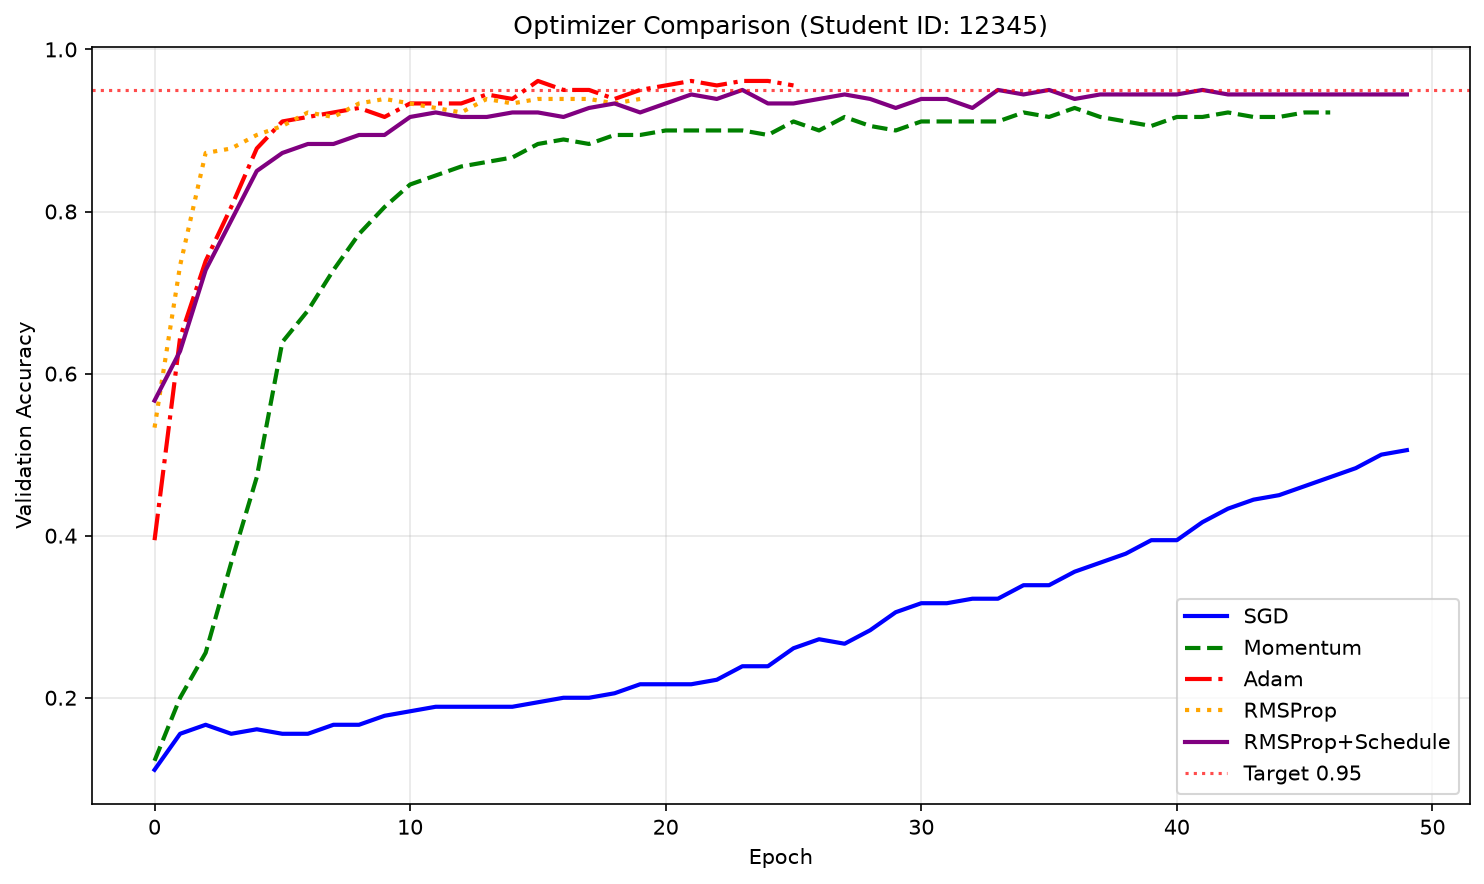
\includegraphics[width=0.85\textwidth]{figures/optimizer_comparison.png}
\caption{Added RMSProp (orange) and RMSProp+Schedule (purple) to the optimizer comparison. RMSProp performs similarly to Adam, and the learning rate schedule helps stabilize training and improves convergence speed.}
\end{figure}

% =====================================================================
% SECTION: BONUS 2
% =====================================================================
\section*{Bonus 2 --- A Normalization Layer [+4]}

I implemented \texttt{BatchNorm1d} as a Tensor layer with train/eval modes.

\subsection*{Implementation}

The layer computes batch statistics during training:
\[
\mu = \frac{1}{N}\sum_i x_i, \quad \sigma^2 = \frac{1}{N}\sum_i (x_i - \mu)^2
\]
\[
\hat{x}_i = \frac{x_i - \mu}{\sqrt{\sigma^2 + \epsilon}}, \quad y_i = \gamma \hat{x}_i + \beta
\]

Running statistics are updated during training and used at evaluation:
\[
\mu_{\text{running}} \leftarrow (1 - \text{momentum}) \cdot \mu_{\text{running}} + \text{momentum} \cdot \mu
\]
\[
\sigma^2_{\text{running}} \leftarrow (1 - \text{momentum}) \cdot \sigma^2_{\text{running}} + \text{momentum} \cdot \sigma^2
\]

\subsection*{Effect on Training}

BatchNorm helps by:
\begin{itemize}
    \item Reducing internal covariate shift
    \item Allowing higher learning rates
    \item Acting as a regularizer
\end{itemize}


% =====================================================================
% SECTION: BONUS 3
% =====================================================================
\section*{Bonus 3 --- Proof of Adam Bias Correction Unbiasedness [+3]}

\subsection*{Problem Statement}

Show that the bias-corrected first moment estimate in Adam:
\[
\hat{m}_t = \frac{m_t}{1-\beta_1^t}
\]
is an unbiased estimate of the expected gradient $\mathbb{E}[g_t]$.

\subsection*{Proof}

Let $g_t$ be the gradient at time step $t$. Adam maintains the first moment estimate:

\[
m_t = \beta_1 m_{t-1} + (1-\beta_1)g_t
\]

where $\beta_1 \in (0, 1)$ is the decay rate, and $m_0 = 0$.

\subsubsection*{Step 1: Unroll the recurrence}

Expanding the recurrence:

\[
m_t = (1-\beta_1) \sum_{i=1}^{t} \beta_1^{t-i} g_i
\]

\subsubsection*{Step 2: Take the expectation}

Under the standard stationarity assumption ($\mathbb{E}[g_i] = \mathbb{E}[g]$ for all $i$):

\[
\mathbb{E}[m_t] = (1-\beta_1) \sum_{i=1}^{t} \beta_1^{t-i} \mathbb{E}[g_i]
= (1-\beta_1) \mathbb{E}[g] \sum_{i=1}^{t} \beta_1^{t-i}
\]

\subsubsection*{Step 3: Evaluate the geometric series}

\[
\sum_{i=1}^{t} \beta_1^{t-i} = \sum_{j=0}^{t-1} \beta_1^{j}
= \frac{1-\beta_1^t}{1-\beta_1}
\]

\subsubsection*{Step 4: Substitute back}

\[
\mathbb{E}[m_t] = (1-\beta_1) \mathbb{E}[g] \cdot \frac{1-\beta_1^t}{1-\beta_1}
= (1-\beta_1^t) \mathbb{E}[g]
\]

\subsubsection*{Step 5: Compute the expectation of the bias-corrected estimate}

\[
\mathbb{E}[\hat{m}_t] = \mathbb{E}\left[\frac{m_t}{1-\beta_1^t}\right]
= \frac{\mathbb{E}[m_t]}{1-\beta_1^t}
= \frac{(1-\beta_1^t) \mathbb{E}[g]}{1-\beta_1^t}
= \mathbb{E}[g]
\]

\subsection*{Conclusion}

\[
\boxed{\mathbb{E}[\hat{m}_t] = \mathbb{E}[g_t]}
\]

Therefore, $\hat{m}_t$ is an \textbf{unbiased estimator} of $\mathbb{E}[g_t]$. Without bias correction, $m_t$ starts at zero and is initially dominated by zero initialization, making early steps much smaller than intended.



% =====================================================================
% SECTION: AI DISCLOSURE
% =====================================================================
\section{AI-use Disclosure}
\begin{center}
\fbox{\parbox{0.9\textwidth}{\centering
\textbf{ChatGPT} -- used for: \\
• Explaining Adam bias correction and RMSProp derivations \\
• Debugging Tensor shape issues in backward passes \\
• Helping structure and format the report \\[0.1in]
All code was written, understood, and verified by me. \\
I can explain everything submitted.
}}
\end{center}

% =====================================================================
% SECTION: REFERENCES
% =====================================================================
\section{References}
\begin{itemize}
    \item Course notes (Weeks 1–2 reading material)
    \item Goodfellow, I., Bengio, Y., & Courville, A. (2016). *Deep Learning*. MIT Press. Ch. 6 (Backpropagation), Ch. 7 (Regularization), Ch. 8 (Optimization)
    \item Kingma, D. P., & Ba, J. (2015). Adam: A Method for Stochastic Optimization. *ICLR 2015*.
    \item RmsProp:
    https://medium.com/@piyushkashyap045/understanding-rmsprop-a-simple-guide-to-one-of-deep-learnings-powerful-optimizers-403baeed9922
    \item SGD with Momentum:
    https://medium.com/@piyushkashyap045/understanding-sgd-with-momentum-in-deep-learning-a-beginner-friendly-guide-0252ede605b4
    \item Learning Rate Scheduling:
    https://machinelearningmastery.com/a-gentle-introduction-to-learning-rate-schedulers/
\end{itemize}

\end{document}